\documentclass[table, 12pt]{article}
\usepackage{graphicx}
\usepackage[T1]{fontenc}
\usepackage{tocloft}
\usepackage{todonotes}
\usepackage{caption}
\usepackage{hyperref}
\usepackage{booktabs}
\usepackage{listings}
\usepackage{pdfpages}
\usepackage{pdflscape}
\usepackage{textpos}
\usepackage{scrhack}
\usepackage{xcolor}
\usepackage{float}
\usepackage{longtable}
\usepackage{enumitem}
\usepackage{tasks}
\usepackage{tabularx}
\usepackage{titlesec}
\usepackage{listing}
\usepackage{graphicx}


\titleformat{\paragraph}
{\normalfont\normalsize\bfseries}{\theparagraph}{1em}{}
\titlespacing*{\paragraph}
{0pt}{3.25ex plus 1ex minus .2ex}{1.5ex plus .2ex}
\begin{document}
\begin{titlepage}
    \centering
    {\scshape\large AY 2020/2021 \par}
    \vfill
    
\includegraphics[width=100pt]{assets/logo-polimi-new}\par\vspace{1cm}
    {\scshape\LARGE Politecnico di Milano \par}
    \vspace{1.5cm}
    {\huge\bfseries Implementation Document \par}
    \vspace{2cm}
    {\Large {Luca Pirovano\quad Nicolò Sonnino}\par}
    \vfill
    {\large Professor\par
        Matteo \textsc{Rossi}}
    \vfill
    {\large \textbf{Version 1.0} \\ \today \par}
\end{titlepage}
\hypersetup{%
    pdfborder = {0 0 0}
}
\thispagestyle{plain}
\pagenumbering{gobble}
\mbox{}
\newpage
\pagenumbering{roman}
\tableofcontents
\newpage
\pagenumbering{arabic}

\section{Introduction}
\subsection{Purpose}
This document aims to describe how the implementation and integration testing took place.
Implementation is the last step of the CLup application development cycle.

Testing, instead, means check that the critical parts of the application works in a correct way, as described in the DD document.

The code and the releases can be find on the official CLup repository hosted on GitHub, reachable at this link:\\ \href{https://github.com/PiroX4256/SE2-Piemonti-Pirovano-Sonnino}{https://github.com/PiroX4256/SE2-Piemonti-Pirovano-Sonnino}.

\subsection{Definitions, Acronyms, Abbreviations}
\subsubsection{Definitions}
\subsubsection{Acronyms}
\begin{itemize}
    \item \textbf{DD:} Design Document
    \item \textbf{RASD:} Requirements Analysis and Specification Document
    \item \textbf{S2B:} Software To Be
    \item \textbf{DTO:} Data Transfer Object, represents a link between the user input and a Java Object.
\end{itemize}
\subsubsection{Abbreviations}
\subsection{Revision history}

\subsubsection{References}
\begin{itemize}
    \item \textbf{JavaScript: } \href{https://www.javascript.com}{https://www.javascript.com}
    \item \textbf{Java: } \href{https://www.java.com/it}{https://www.java.com/it}
    \item \textbf{Spring Framework: } \href{https://spring.io}{https://spring.io}
    \item \textbf{Spring Security: } \href{https://spring.io/projects/spring-security}{https://spring.io/projects/spring-security}
    \item \textbf{Spring Social: } \href{https://projects.spring.io/spring-social}{https://projects.spring.io/spring-social}
    \item \textbf{Vue.js: } \href{https://vuejs.org}{https://vuejs.org}
    \item \textbf{jQuery: } \href{https://jquery.com}{https://jquery.com}
    \item \textbf{QRcode.js: } \href{https://jquery.com}{https://jquery.com}
    \item \textbf{Semantic UI: } \href{https://semantic-ui.com}{https://semantic-ui.com}
    \item \textbf{Leaflet.js} \href{https://leafletjs.com}{https://leafletjs.com}
    \item \textbf{} \href{}{}
\end{itemize}

\newpage
\section{Development}
\subsection{Implemented Functionalities}
With respect to the RASD and DD documents, we decided to implement the following functions:
\begin{itemize}
    \item \textbf{Sign Up}
    \item \textbf{ASAP: As Soon As Possible}
    \item \textbf{Hand out tickets on spot}
\end{itemize}
For more details regarding the specific functionalities, you are invited to read the RASD document, which contains a very detailed description of them.

We chooses to implement these functionalities in order to simulate a Module 1 product purchase. In fact, we remind that the application is divided into three modules; the first one is also called \textit{MVP}, and contains the basic functionalities of CLup, the second one contains the \textit{Book a Visit} feature and the last one includes the custom deploy on organization's servers.

In a real-world scenario, the most used module would be of course the first one (due to its simplicity), so that we decided to focus on it.

\subsection{Adopted Development Frameworks}
As we said in our DD, the application should follow a four-tier architecture, with a fully REST interface and a lot of client scripting. Finally, we decided to adopt the Model-View-Controller pattern, which is one of the most used in distributed applications.

In the following pages you will find a list of adopted frameworks and technologies in order to accomplish to this requirements.

\subsubsection{Programming languages}
For sake of standards and application speed we decided to use the Java\texttrademark  Programming Language, which is one of the most used languages in web and distributed applications.

Of course, there are some pros and cons about using this type of language:
\\\begin{itemize}
    \item \textbf{Pros:}
          \begin{itemize}
              \item[+] Speed: of course, since it is a compiled language, Java permits to have very good performances on these elaborations;
              \item[+] Standard: as shown in figure \ref{languages_comparison}, Java is the \textit{De Facto standard} in enterprise web development and represents a very good solution for portable applications;
              \item[+] Stability: Java is a mature language that has immensely evolved over the years. Hence it’s more stable and predictable.
              \item[+] Object-Oriented: The object-oriented nature of Java allows developers to create modular programs and write reusable codes. This saves lots of efforts and time, improving the productivity of the development process.
              \item[+] Well-documented
          \end{itemize}
    \item \textbf{Cons:}
          \begin{itemize}
              \item High verbosity: with respect to other programming languages (such as Python), Java contains a more verbose and less-readable syntax.
              \item High memory consumption: since Java Programs run on top of Java Virtual Machine, it consumes more memory.
          \end{itemize}
\end{itemize}

For the client-side scripting, we decided to adopt JavaScript\texttrademark  for the web app, and Flutter with Dart\texttrademark  language for the mobile app.

JavaScript is a text-based programming language used both on the client-side and server-side that allows to make web pages interactive. Where HTML and CSS are languages that give structure and style to web pages, JavaScript gives web pages interactive elements that engage a user.

Flutter, instead, is an open-source UI software development kit created by Google. It is mostly used to develop applications for Android and iOS.

\begin{figure}[H]
    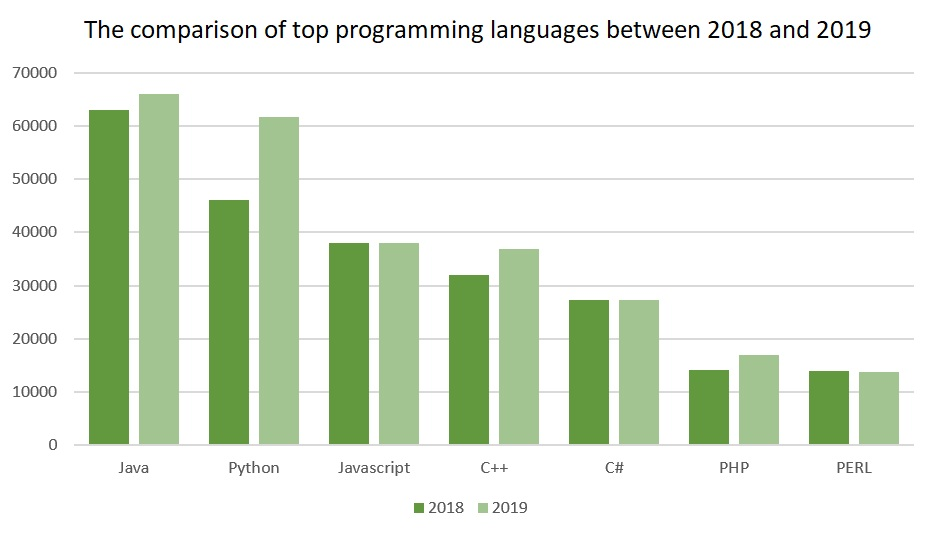
\includegraphics[width=\textwidth]{assets/graph-18-19-languages.jpg}
    \caption{Web Programming languages usage (2018 vs 2019)}
    \label{languages_comparison}
\end{figure}

\begin{figure}[H]
    
\includegraphics[width=\textwidth]{assets/client-side-scripting.png}
    \caption{Client-side technologies}
\end{figure}

\subsection{Java Frameworks}
\subsubsection{Spring}
\label{spring}
In order to accomplish the S2B requirements, we decided to adopt the Spring development framework.

Spring is an open source framework, used for RESTful Java application development. It's built on top of the Java Enterprise Edition (JEE) and represents an efficient and modern alternative to the classic Enterprise Java Bean (EJB) model.

Of course, using a framework means works on a solid base, which is well tested and documented. In fact, Spring contains a proper paradigm in order to build web services on its API.

\begin{figure}
    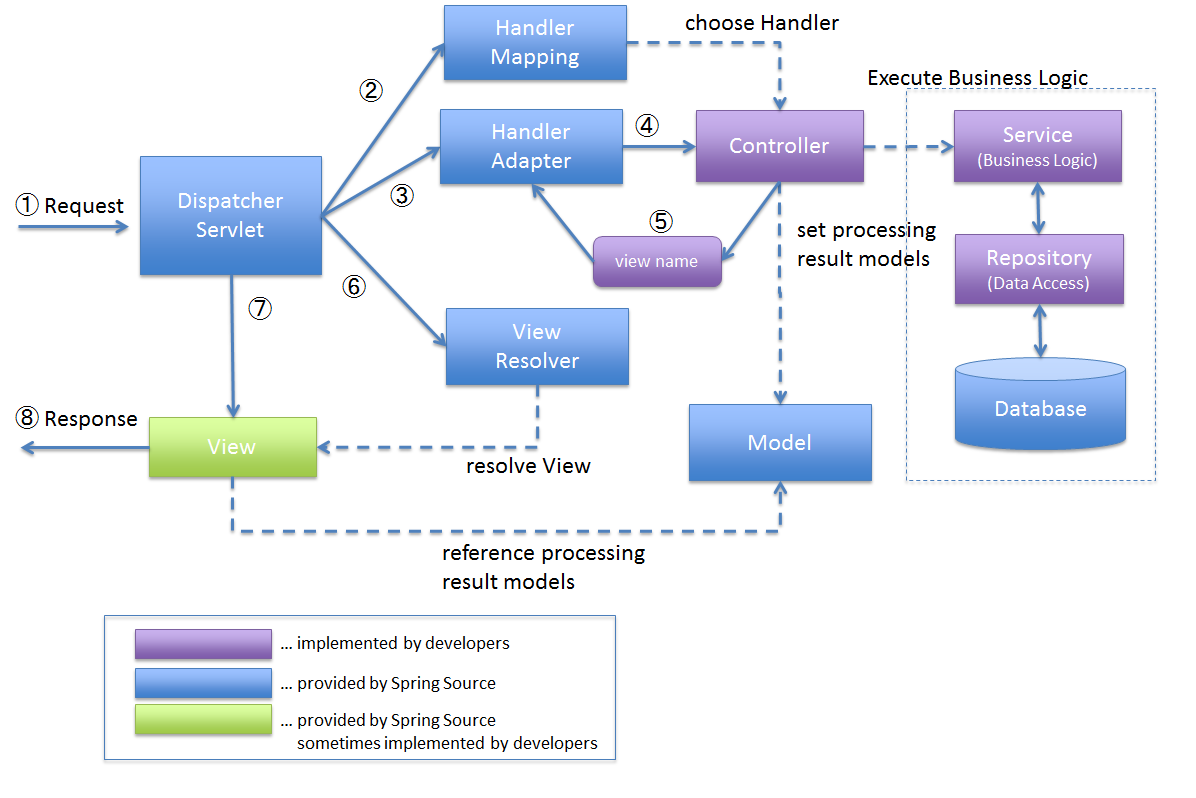
\includegraphics[width=\textwidth]{assets/SpringArchitecture.png}
    \caption{Spring Framework architecture}
    \label{spring_architecture}
\end{figure}

As shown in figure \ref{spring_architecture}, the architecture of Spring is very simple and easy-to-use.

In fact, it is composed by:
\begin{itemize}
    \item \textbf{Dispatcher Servlet:} its job is to route all the incoming requests to the correct Spring controller, which is properly mapped with an appropriate annotation. This is done through the severals components of Spring, which are HandlerMapping, HandlerAdapter and ViewResorver.
    \item \textbf{Controller:} the controller acts as an interface between the user and the services. It catches the requests coming from the dispatcher and makes actions relying on what user passed to it.
    \item \textbf{Model:} it contains the application logic about the transfer objects (also called DTO) which maps a user input (which is encoded in JSON format) and a Java object. The DTOs can also be used in the opposite direction (server to client), so they are encoded in JSON format and then sent to the client.
    \item \textbf{Services:} they act as an intermediate between the entities (database objects) and the controller, containing some useful methods in order to manipulate data sent by controllers.
    \item \textbf{Repositories:} they are interfaces that contains the query methods in order to fetch data from database. They are managed from Spring engine and it suffices to specify what to retrieve in order to get a response object from the DBMS.
    \item \textbf{Entities:} they represent database objects. They are declared with @Entity annotation, which maps the object to a database table (or set of them). Inside an entity object it is possible to specify constraints and foreign references through proper annotations.
\end{itemize}

\subsubsection{Spring Data JPA}
Spring Data JPA, part of the larger Spring Data family, permits to easily implement JPA based repositories. This module deals with enhanced support for JPA based data access layers. It makes it easier to build Spring-powered applications that use data access technologies.

Spring Data JPA aims to significantly improve the implementation of data access layers by reducing the effort to the amount that’s actually needed.

In fact, through services and repositories, interfacing with the database becomes very simple. Useless to say that, furthermore, the security of the queries from SQL injection is high, because it is totally managed by Spring.

\subsubsection{Spring Security}
Spring Security is a plugin of the Spring Mvc suite, which manages the application security.

In fact, it is role-based and permits, through several annotations, to grant access to controller only to authorized people.

In CLup, Spring Security is also the responsible for the REST authentication, which is made through a pattern called JWT (Json Web Token).

Practically, it is an open standard (RFC 7519) that defines a compact and self-contained way for securely transmitting information between parties as a JSON object.
In our case, there is an exchange of a token which authorizes each client request, so the client needs to attach it to request's headers each time it calls the server.
\subsubsection{Spring Social}
Spring Social is another plugin of the Spring family which permits the user authentication through several identity providers (IdPs).

For sake of simplicity, we decided to start from the Facebook one, which is one of the most used social network nowadays. Once called, Facebook servers authenticate the user and return back to the CLup backend its information, which generally consists of name, surname and profile id.

Obviously, the same can be done with the other identity providers, such as Google, Twitter, GitHub, etc.

\subsection{Other Frameworks}
\label{client_side_frameworks}
\subsubsection{Vue.js}
Vue is a progressive framework for building user interfaces. Unlike other monolithic frameworks, Vue is designed from the ground up to be incrementally adoptable. The core library is focused on the view layer only, and is easy to pick up and integrate with other libraries or existing projects. On the other hand, Vue is also perfectly capable of powering sophisticated Single-Page Applications when used in combination with modern tooling and supporting libraries.

We used Vue.js to manage the client-side rendering of the pages on the web app. In fact, each page calls its scripts, which are responsible for the correct orchestration.
\subsubsection{jQuery}
jQuery is a fast, small, and feature-rich JavaScript library. It makes things like HTML document traversal and manipulation, event handling, animation, and Ajax much simpler with an easy-to-use API that works across a multitude of browsers. With a combination of versatility and extensibility, jQuery has changed the way that millions of people write JavaScript.

We used jQuery to implement the network layer of the client-side web application. In fact, it is responsible (through the Ajax plugin) of the communication with the server, managing all the requests and response.

\subsubsection{QRcode.js}
QRCode.js is javascript library for making QRCode. QRCode.js supports Cross-browser with HTML5 Canvas and table tag in DOM. QRCode.js has no dependencies.

We used this library in order to generate a visual representation, through a Quick Response Code (also known as QRCode), of the ticket unique id, in order to easily permit its validation at the supermarket entrance.

\subsubsection{Semantic UI}
Semantic UI is a graphical framework which is useful to construct good-looking web interfaces with less effort than making them manually.

It includes several css styles, together with a full JavaScript set of functionalities (such as dynamic management of the page).
\subsection{API Integrations}
\subsubsection{Leaflet.js}
Leaflet is an open source JavaScript library used to build web mapping applications.

We used it to render the maps containing stores position, in the user and manager private area.

\newpage
\section{Source Code}
\subsection{Backend}
The backend is packaged through the Maven framework, which gives also a standard for organizing the code. Of course, we followed this standard, merged with the Spring Framework one.

More details about the maven projects standard organization can be found at \href{https://maven.apache.org/guides/introduction/introduction-to-the-standard-directory-layout.html}{https://maven.apache.org/guides/introduction/introduction-to-the-standard-directory-layout.html}
\subsubsection{Packages}
As previously said, the application backend is built on top of the Spring Framework, which follows an architectural pattern called Model View Controller (MVC). The extension of the MVC provided by Spring defines also a standard structure of the project classes.

\subsubsection*{Package it.polimi.se2.clupapplication}
\begin{itemize}
    \item \textbf{Config:} this package contains the configuration classes of Spring framework, which manage security and general application configuration.
    \item \textbf{Controllers:} it contains all the controllers of CLup application, following the Spring controllers paradigm. See section \ref{spring_architecture} for more details.
    \item \textbf{Entities:} this package contains all the relational database objects, which are properly mapped to a SQL server through the JPA APIs. Each table has its own entity class, with the exception of the bridge (OneToOne, OneToMany, ManyToMany) relations.
    \item \textbf{Model:} following Spring standard, this package includes all the DTO (Data Transfer Objects) for data exchange between client and server.
    \item \textbf{Repositories:} it contains the Spring repositories, which are the interfaces required in order to query the DBMS and the related entities.
    \item \textbf{Security:} part of the Spring plugins, this package includes the security classes of CLup application. In fact, these classes manages the process of login and signup through the exchange of the JWT (Json Web Token). Furthermore, they also implement the IdP sign in feature with social networks (such as Facebook).
    \item \textbf{Services:} this last package contains the service classes, which are the intermediates between controllers and repositories, following the Spring approach described in section \ref{spring_architecture}.
\end{itemize}

\subsubsection{Flow of a request}
\begin{figure}[H]
    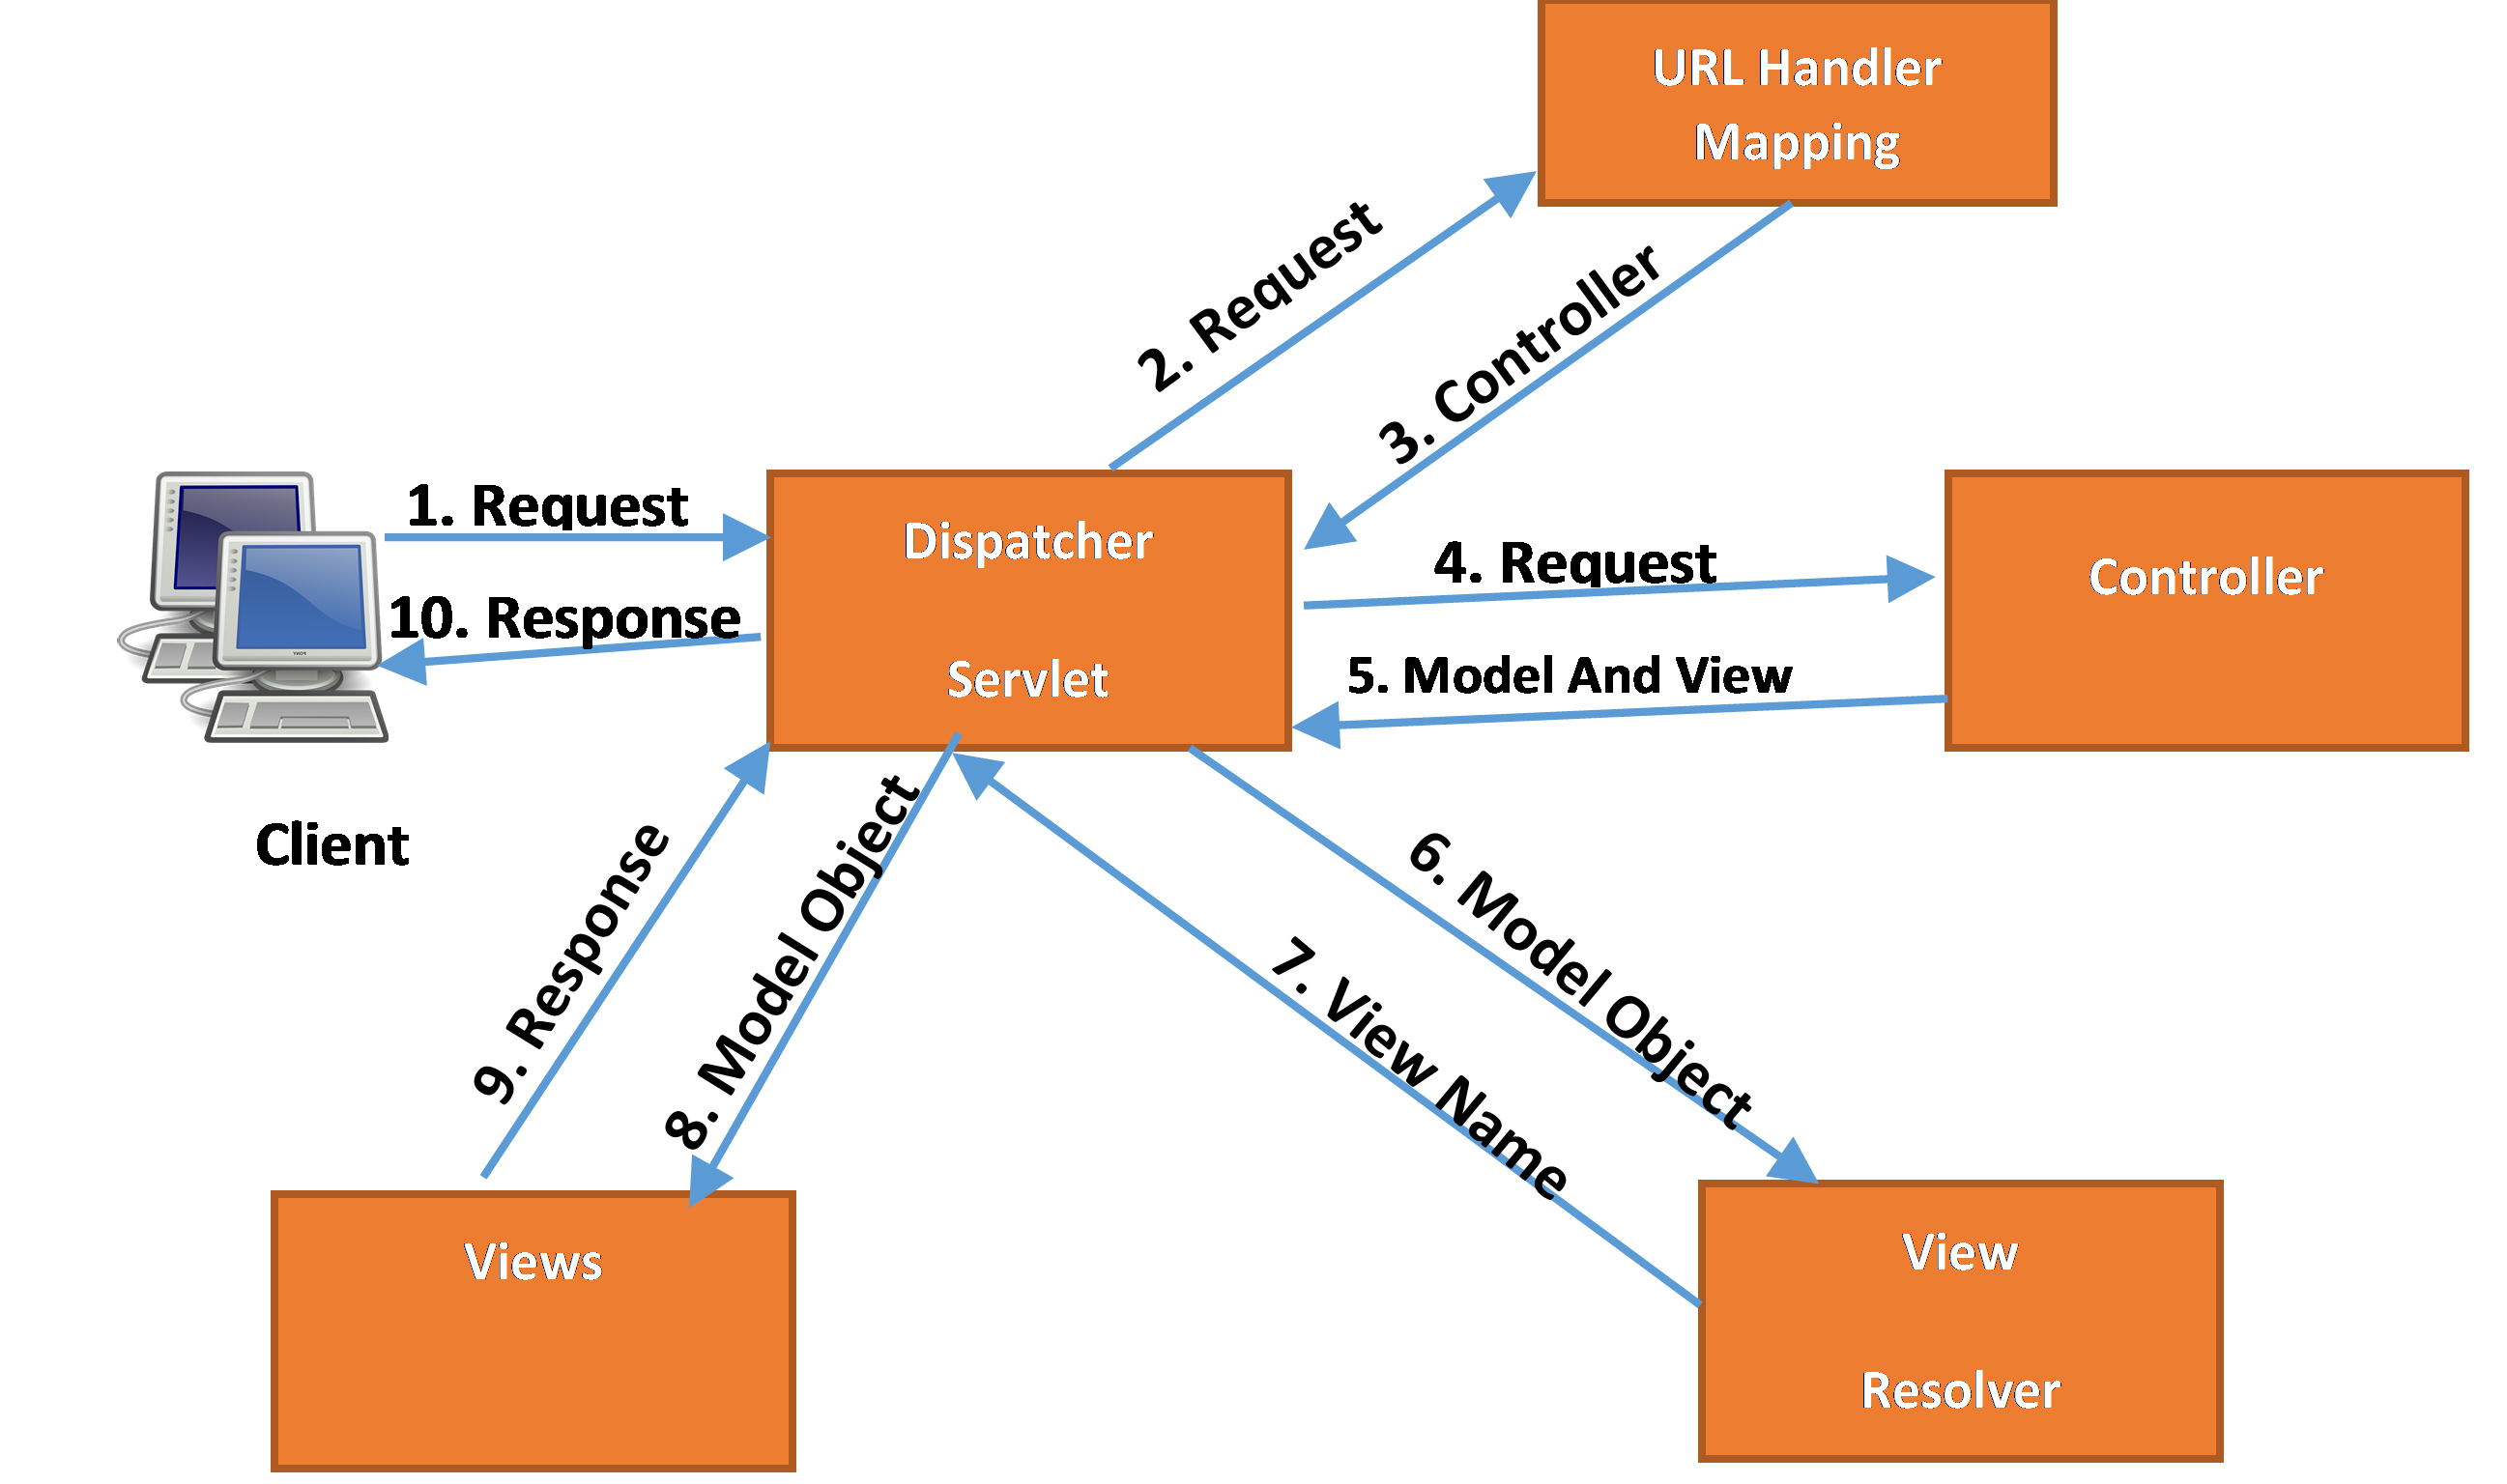
\includegraphics[width=\textwidth]{assets/Spring-MVC-Flow-Diagram.jpg}
    \caption{Flow of a client request to backend}
    \label{spring_mvc_request}
\end{figure}
As you can see in figure \ref{spring_mvc_request}, a request coming from a client follows several step into the backend structure.

First of all, it is intercepted by the Dispatcher Servlet, which forwards the request to the URL Handler Mapping. This handler contains the mapped urls from all the application controller and also the method accepted (GET, POST, PUT, etc.).

Once URL Handler has resolved the associated controller, the request is dispatched to the correct controller, which calls the classes needed for elaboration (such as services and, consequently, repositories).

After the elaboration, the controller creates a ResponseEntity object and sends it to the view resolver which, with the help of Views class, return the response to Dispatcher Servlet.

Finally, the Dispatcher Servlet return the created response to the client.

\subsubsection{Test cases}
The test cases, which are described in details in section \ref{testing}, are located under the maven \textit{test} folder, into the package it.polimi.se2.clupapplication.

\subsection{Frontend Structure}
\subsubsection{Web Application}
The front-end web application is contained into the \textit{resources/public} folder of the Spring application, in order to permit an easy reachability directly from the backend dispatcher without being filtered from the security manager.
Of course, following the four tier architecture described in the Design Document, the front-end web application can also be deployed to a dedicated web server, which will then make requests to a different backend server.

The structure of the web app is the following:
\begin{itemize}
    \item \textbf{admin:} this folder contains all the administration HTML web pages, which are served with the \textit{/admin} url prefix;
    \item \textbf{attendant:} this folder, instead, contains all the attendant dashboard HTML web pages, which are served with the \textit{/attendant} url prefix;
    \item \textbf{static:} this last folder contains all the static files of the web application, which consists of CSS stylesheets, JS scripts, fonts, images and client-side frameworks adopted (see section \ref{client_side_frameworks});
    \item all the other HTML files in \textit{public} directory refer to the customer web interface, which will be of course the most used pages.
\end{itemize}
\subsubsection{Mobile App}

\subsection{Other Useful Information}
The application is configured to fetch data from a MySQL database, which credentials must be specified in the application.yaml properties file. This configuration file can be found in \textit{resources} folder and contains also all the other static configurations of the application, such as jpa configurations, social login credentials, jwt token settings, etc.
\newpage
\section{Testing}
\label{testing}
\subsection{Backend}

\subsection{Mobile Application}

\newpage
\section{Installation Instructions}

\section{Effort spent}
\begin{center}
    \begin{tabular}{ | c || c | c | c | c| c|}
        \hline
        Student        & Time for Implementation Project \\ \hline
        Luca Pirovano  & 50 hours                        \\ \hline
        Nicolò Sonnino & 3h                              \\
        \hline
    \end{tabular}
\end{center}
\end{document}